\chapter{PK2 --- Quyền riêng tư}
\begin{figure}[H]\centering
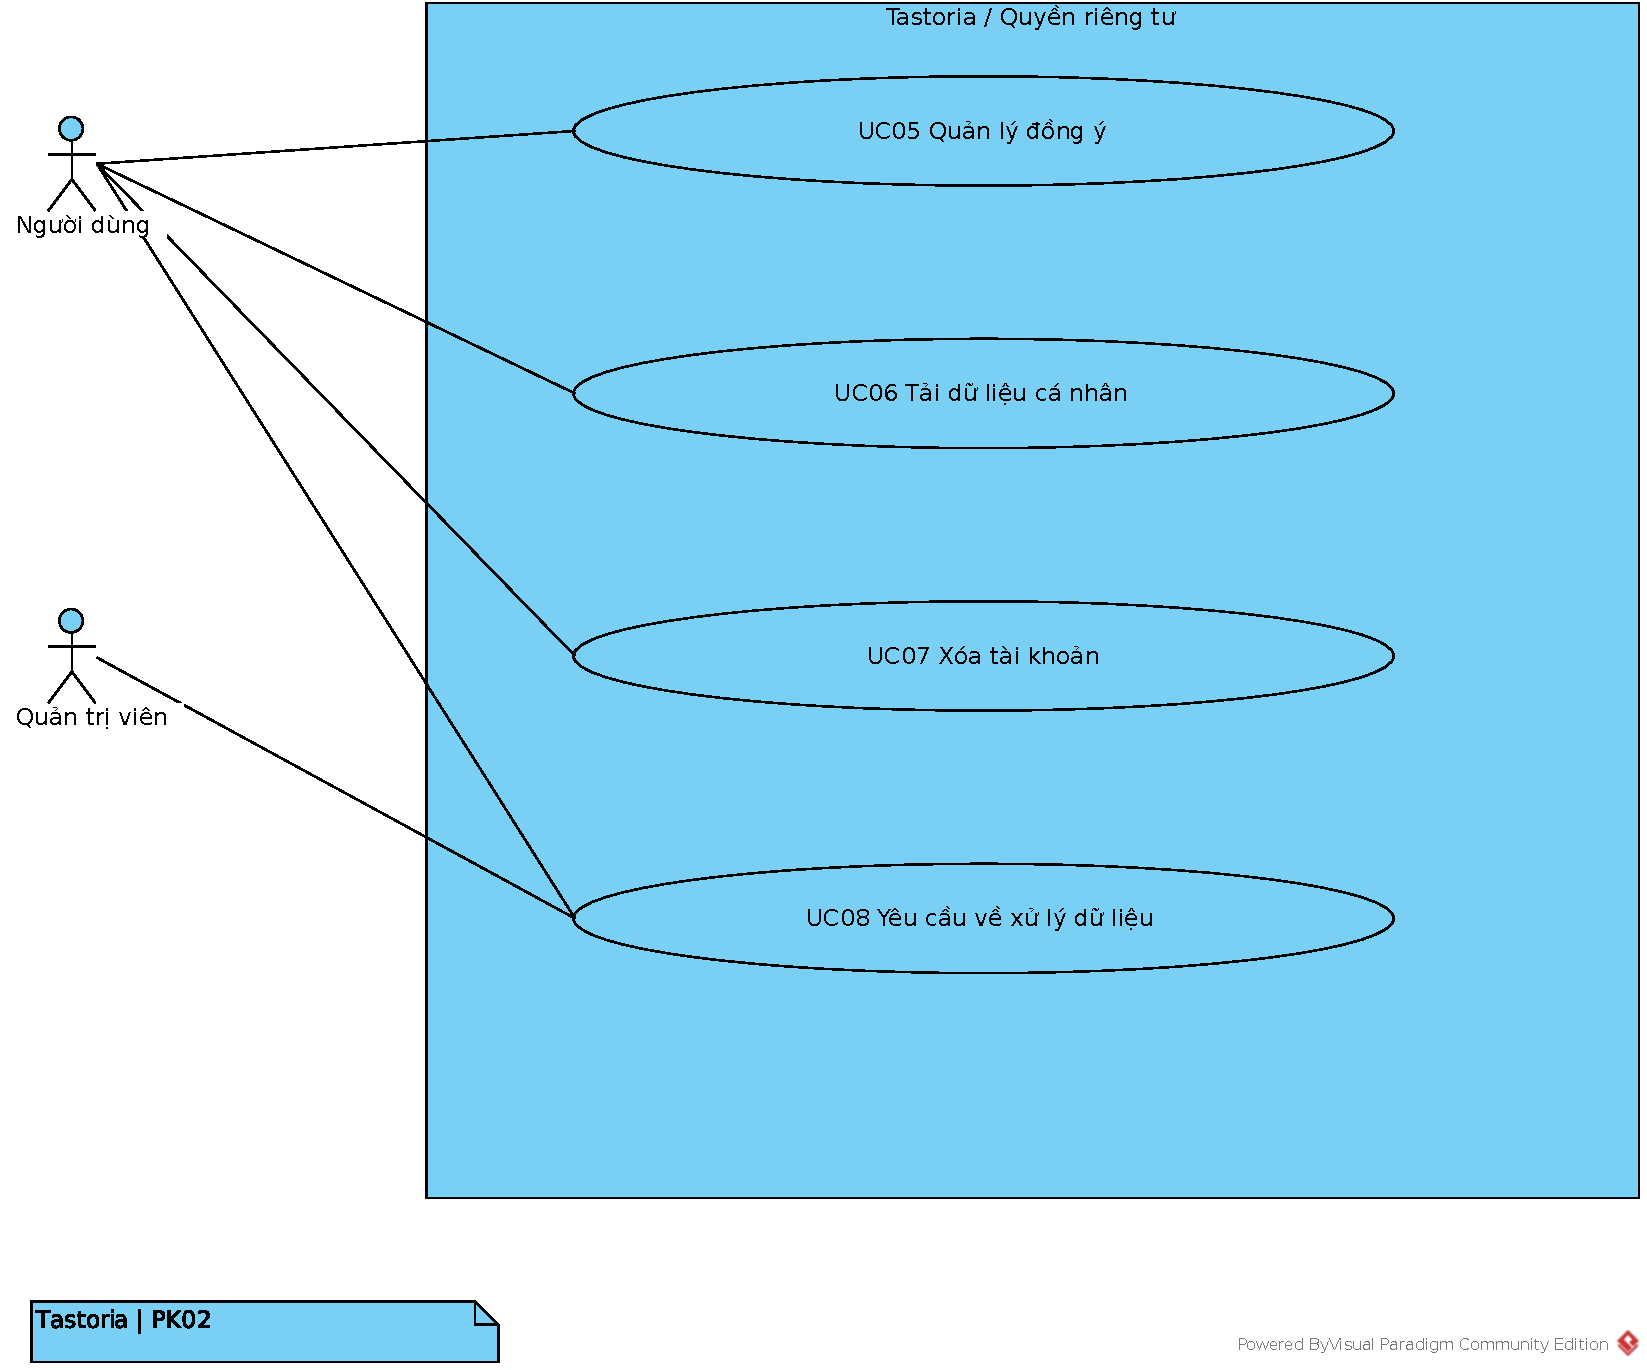
\includegraphics[width=0.96\linewidth,height=0.75\textheight,keepaspectratio]{assets/PK02.pdf}
\caption{PK02 --- Phân rã use case}\label{fig:Phu-luc-A-Use-Cases:2}
\end{figure}
\section{UC05 --- Quản lý đồng ý theo mục đích}
\subsection{Mục tiêu trong ngữ cảnh}
Người dùng (A02) xem từng mục đích xử lý dữ liệu, đồng ý hoặc rút đồng ý cho từng mục đích riêng, và biết hệ thống sẽ làm gì với dữ liệu khi rút. Hệ thống giữ nhật ký đồng ý chỉ ghi thêm, gắn với phiên bản điều khoản đã hiển thị. Chức năng đồng ý được truy cập trong luồng UC09 theo lựa chọn người dùng và từ Cài đặt; không mô hình hóa toàn bộ UC05 là include bắt buộc.

\subsection{Phạm vi và mức}
\begin{itemize}
\item Phạm vi: hệ thống Tastoria, module {\small\texttt{privacy}} (M03); {\small\texttt{privacy}} gọi {\small\texttt{identity}} (M02) để tăng {\small\texttt{token\_\allowbreak{}\allowbreak{}version}}. Việc xoá dữ liệu theo mục đích chạy trong worker và gọi các bộ xoá mà module {\small\texttt{profile}}, {\small\texttt{events}}, {\small\texttt{scan}} đã đăng ký với sổ đăng ký dữ liệu cá nhân của {\small\texttt{core}} (M01), nên {\small\texttt{privacy}} không phụ thuộc ngược vào các module đó.
\item Mức: mục tiêu người dùng.
\item Mục đích áp dụng cho A02: {\small\texttt{health\_\allowbreak{}\allowbreak{}profile}}, {\small\texttt{personalization}}, {\small\texttt{photo\_\allowbreak{}\allowbreak{}contribution}}. Mục đích {\small\texttt{survey}} dành cho Người tham gia khảo sát (A03) ở UC23, không quản lý ở UC này.
\end{itemize}
\subsection{Tác nhân và bên liên quan (quyền lợi)}
{\footnotesize\setlength{\tabcolsep}{0pt}
\begin{longtable}{@{}L{7.850cm}@{\hspace{3mm}}L{7.850cm}@{}}
\caption{Tác nhân và bên liên quan (quyền lợi)}\\
\toprule
\textbf{Tác nhân /\allowbreak{} bên liên quan} & \textbf{Quyền lợi} \\
\midrule\endfirsthead
\multicolumn{2}{l}{\small\itshape Bảng \thetable{} (tiếp theo)}\\
\toprule
\textbf{Tác nhân /\allowbreak{} bên liên quan} & \textbf{Quyền lợi} \\
\midrule\endhead
\bottomrule\endfoot
A02 Người dùng (chính) & Chọn riêng từng mục đích, không bị tích sẵn; rút lúc nào cũng được và có hiệu lực ngay. \\ \addlinespace[3pt]
Nhóm vận hành /\allowbreak{} bên kiểm tra tuân thủ & Chứng minh được ai đồng ý mục đích nào, với văn bản điều khoản nào, lúc nào, qua kênh nào (Luật 91/\allowbreak{}2025, NĐ 356/\allowbreak{}2025). \\ \addlinespace[3pt]
Các module dùng dữ liệu ({\small\texttt{profile}}, {\small\texttt{events}}, {\small\texttt{meal}}, {\small\texttt{scan}}) & Có một nguồn trả lời duy nhất "người này hiện có đồng ý mục đích X không". \\ \addlinespace[3pt]
\end{longtable}}
\subsection{Tiền điều kiện}
\begin{itemize}
\item A02 đã đăng nhập.
\item Mỗi mục đích có ít nhất một {\small\texttt{policy\_\allowbreak{}\allowbreak{}versions}} với {\small\texttt{effective\_\allowbreak{}\allowbreak{}from \ensuremath{\leq} now()}}.
\end{itemize}
\subsection{Đảm bảo tối thiểu}
\begin{itemize}
\item {\small\texttt{consent\_\allowbreak{}\allowbreak{}events}} chỉ được thêm dòng; không có UPDATE hay DELETE (trừ xoá dây chuyền khi xoá tài khoản ở UC07).
\item Không có đồng ý nào được ghi mà người dùng chưa chủ động bật.
\item Sau khi rút, không module nào được tiếp tục dùng dữ liệu của mục đích đó, kể cả khi việc xoá dữ liệu chưa chạy xong.
\end{itemize}
\subsection{Đảm bảo khi thành công}
\begin{itemize}
\item Đồng ý: có {\small\texttt{consent\_\allowbreak{}\allowbreak{}events}} {\small\texttt{action = grant}} trỏ {\small\texttt{policy\_\allowbreak{}\allowbreak{}versions}} hiện hành; {\small\texttt{v\_\allowbreak{}\allowbreak{}current\_\allowbreak{}\allowbreak{}consents}} trả {\small\texttt{granted}}.
\item Rút: có {\small\texttt{consent\_\allowbreak{}\allowbreak{}events}} {\small\texttt{action = withdraw}}; {\small\texttt{users.\allowbreak{}token\_\allowbreak{}\allowbreak{}version}} tăng 1; có {\small\texttt{dsr\_\allowbreak{}\allowbreak{}requests}} {\small\texttt{type = withdraw}}; trong \ensuremath{\leq} 24 giờ dữ liệu của mục đích bị xoá và yêu cầu chuyển {\small\texttt{completed}}.
\end{itemize}
\subsection{Kích hoạt}
\begin{itemize}
\item A02 tới màn đồng ý trong Hồ sơ 60 giây (UC09, {\small\texttt{channel = onboarding}}), hoặc mở Cài đặt > Đồng ý ({\small\texttt{channel = settings}}).
\item App phát hiện một mục đích ở trạng thái {\small\texttt{superseded}} (điều khoản có bản mới) khi mở app.
\end{itemize}
\subsection{Kịch bản chính}
\begin{enumerate}
\item App gọi {\small\texttt{GET /\allowbreak{}\allowbreak{}me/\allowbreak{}\allowbreak{}consents}}; module {\small\texttt{privacy}} đọc {\small\texttt{v\_\allowbreak{}\allowbreak{}current\_\allowbreak{}\allowbreak{}consents}} và trả trạng thái của từng mục đích ({\small\texttt{none}}, {\small\texttt{granted}}, {\small\texttt{withdrawn}}, {\small\texttt{superseded}}).
\item Với mỗi mục đích, app gọi {\small\texttt{GET /\allowbreak{}\allowbreak{}policies/\allowbreak{}\allowbreak{}\{purpose\}/\allowbreak{}\allowbreak{}current}}; {\small\texttt{privacy}} trả bản điều khoản hiện hành từ {\small\texttt{policy\_\allowbreak{}\allowbreak{}versions}} và {\small\texttt{consent\_\allowbreak{}\allowbreak{}purposes}} ({\small\texttt{name\_\allowbreak{}\allowbreak{}vi}}, {\small\texttt{description\_\allowbreak{}\allowbreak{}vi}}, {\small\texttt{data\_\allowbreak{}\allowbreak{}category}}, {\small\texttt{is\_\allowbreak{}\allowbreak{}sensitive}}, {\small\texttt{version}}, {\small\texttt{text\_\allowbreak{}\allowbreak{}sha256}}, nội dung).
\item App hiện mỗi mục đích một công tắc riêng kèm mô tả và hệ quả khi không bật; mọi công tắc chưa có {\small\texttt{granted}} hiển thị ở trạng thái tắt.
\item A02 bật các mục đích muốn đồng ý và bấm "Lưu".
\item App gửi {\small\texttt{POST /\allowbreak{}\allowbreak{}me/\allowbreak{}\allowbreak{}consents}} với danh sách {\small\texttt{\{purpose, policy\_\allowbreak{}\allowbreak{}version\_\allowbreak{}\allowbreak{}id\}}} vừa bật, {\small\texttt{channel}}, {\small\texttt{app\_\allowbreak{}\allowbreak{}version}}.
\item Module {\small\texttt{privacy}} kiểm từng {\small\texttt{policy\_\allowbreak{}\allowbreak{}version\_\allowbreak{}\allowbreak{}id}} là bản hiện hành của mục đích tương ứng, ghi một {\small\texttt{consent\_\allowbreak{}\allowbreak{}events}} {\small\texttt{action = grant}} cho mỗi mục đích chưa ở trạng thái {\small\texttt{granted}} với đúng bản đó, rồi trả trạng thái mới.
\item Để rút, A02 tắt một công tắc đang bật; app hiện hộp xác nhận nêu dữ liệu sẽ bị xoá trong \ensuremath{\leq} 24 giờ.
\item A02 xác nhận; app gửi {\small\texttt{POST /\allowbreak{}\allowbreak{}me/\allowbreak{}\allowbreak{}consents/\allowbreak{}\allowbreak{}\{purpose\}/\allowbreak{}\allowbreak{}withdraw}}.
\item Module {\small\texttt{privacy}}, trong một giao dịch: ghi {\small\texttt{consent\_\allowbreak{}\allowbreak{}events}} {\small\texttt{action = withdraw}}; gọi {\small\texttt{identity.\allowbreak{}bump\_\allowbreak{}\allowbreak{}token\_\allowbreak{}\allowbreak{}version(user\_\allowbreak{}\allowbreak{}id)}}; tạo {\small\texttt{dsr\_\allowbreak{}\allowbreak{}requests}} {\small\texttt{type = withdraw}}, {\small\texttt{status = received}}, {\small\texttt{subject\_\allowbreak{}\allowbreak{}ref = HMAC-\allowbreak{}SHA256(user\_\allowbreak{}\allowbreak{}id)}}, {\small\texttt{received\_\allowbreak{}\allowbreak{}at = now()}}, {\small\texttt{acknowledged\_\allowbreak{}\allowbreak{}at = now()}}, {\small\texttt{note}} = mã mục đích; xếp job xoá theo mục đích vào worker; commit và trả 200 kèm trạng thái mới và id yêu cầu.
\item App nhận 401 {\small\texttt{token\_\allowbreak{}\allowbreak{}revoked}} ở yêu cầu kế tiếp, tự làm mới phiên (UC02) và nhận access token mang {\small\texttt{token\_\allowbreak{}\allowbreak{}version}} mới.
\item Worker chạy job: {\small\texttt{privacy}} đặt {\small\texttt{dsr\_\allowbreak{}\allowbreak{}requests.\allowbreak{}status = in\_\allowbreak{}\allowbreak{}progress}}, gọi các bộ xoá đã đăng ký cho mục đích đó:\begin{itemize}
\item {\small\texttt{health\_\allowbreak{}\allowbreak{}profile}}: module {\small\texttt{profile}} đặt {\small\texttt{sex\_\allowbreak{}\allowbreak{}enc}}, {\small\texttt{birth\_\allowbreak{}\allowbreak{}year\_\allowbreak{}\allowbreak{}enc}}, {\small\texttt{height\_\allowbreak{}\allowbreak{}cm\_\allowbreak{}\allowbreak{}enc}}, {\small\texttt{weight\_\allowbreak{}\allowbreak{}kg\_\allowbreak{}\allowbreak{}enc}}, {\small\texttt{enc\_\allowbreak{}\allowbreak{}key\_\allowbreak{}\allowbreak{}id}}, {\small\texttt{kcal\_\allowbreak{}\allowbreak{}target}}, {\small\texttt{kcal\_\allowbreak{}\allowbreak{}source}} của {\small\texttt{profiles}} về NULL.
\item {\small\texttt{personalization}}: module {\small\texttt{events}} xoá mọi {\small\texttt{interactions}} của người dùng.
\item {\small\texttt{photo\_\allowbreak{}\allowbreak{}contribution}}: module {\small\texttt{scan}} đặt {\small\texttt{scan\_\allowbreak{}\allowbreak{}images.\allowbreak{}contributed = false}} và xoá tệp trong thư mục {\small\texttt{contrib/\allowbreak{}\allowbreak{}}}; ảnh gốc còn lại theo hạn 30 ngày của BR-\allowbreak{}RETAIN-\allowbreak{}01 (UC32).
\end{itemize}


\item {\small\texttt{privacy}} đặt {\small\texttt{status = completed}}, {\small\texttt{completed\_\allowbreak{}\allowbreak{}at = now()}}.
\end{enumerate}
\subsection{Mở rộng}
\begin{itemize}
\item \textbf{1a. Một mục đích ở trạng thái {\small\texttt{superseded}}:} app hiện văn bản điều khoản mới, nêu đây là bản mới, và yêu cầu bật lại; trong lúc chờ, {\small\texttt{privacy.\allowbreak{}has\_\allowbreak{}\allowbreak{}consent()}} trả false cho mục đích đó (FR-\allowbreak{}05-\allowbreak{}07).
\item \textbf{2a. Mục đích không tồn tại trong {\small\texttt{consent\_\allowbreak{}\allowbreak{}purposes}}:} trả 404 {\small\texttt{code = purpose\_\allowbreak{}\allowbreak{}not\_\allowbreak{}\allowbreak{}found}}.
\item \textbf{4a. A02 không bật mục đích nào và bấm "Lưu" (thiếu đồng ý):} app không gửi {\small\texttt{POST /\allowbreak{}\allowbreak{}me/\allowbreak{}\allowbreak{}consents}}; trạng thái giữ {\small\texttt{none}}. App nêu hệ quả bằng chữ: không có {\small\texttt{health\_\allowbreak{}\allowbreak{}profile}} thì "chưa có mục tiêu" năng lượng (BR-\allowbreak{}CONSENT-\allowbreak{}02); không có {\small\texttt{personalization}} thì gợi ý dựa trên trung bình món và 5 món hay ăn (BR-\allowbreak{}CONSENT-\allowbreak{}03). Luồng UC09 vẫn đi tiếp.
\item \textbf{6a. {\small\texttt{policy\_\allowbreak{}\allowbreak{}version\_\allowbreak{}\allowbreak{}id}} không phải bản hiện hành (điều khoản vừa đổi trong lúc A02 đọc):} trả 409 {\small\texttt{code = policy\_\allowbreak{}\allowbreak{}outdated}}, không ghi dòng nào; app tải lại bản hiện hành (bước 2) và hỏi lại.
\item \textbf{6b. Mục đích đã {\small\texttt{granted}} với đúng bản hiện hành (gửi lại do mất mạng):} {\small\texttt{privacy}} không ghi dòng mới cho mục đích đó và trả 200 với trạng thái hiện tại (lũy đẳng).
\item \textbf{6c. Gửi mục đích {\small\texttt{survey}} hoặc mã lạ:} trả 422 {\small\texttt{code = purpose\_\allowbreak{}\allowbreak{}not\_\allowbreak{}\allowbreak{}allowed}}; không ghi dòng nào cho cả yêu cầu.
\item \textbf{9a. Mục đích đang ở {\small\texttt{none}} hoặc {\small\texttt{withdrawn}} (gửi lại do mất mạng, hoặc rút hai lần):} {\small\texttt{privacy}} trả 200 với trạng thái hiện tại, không ghi {\small\texttt{consent\_\allowbreak{}\allowbreak{}events}}, không tăng {\small\texttt{token\_\allowbreak{}\allowbreak{}version}}, không tạo {\small\texttt{dsr\_\allowbreak{}\allowbreak{}requests}} mới (lũy đẳng).
\item \textbf{9b. Lỗi CSDL ở bước 9:} giao dịch rollback; không có sự kiện rút, {\small\texttt{token\_\allowbreak{}\allowbreak{}version}} không đổi; trả 5xx; công tắc trên app quay về bật và app cho thử lại.
\item \textbf{11a. Job xoá lỗi:} worker thử lại theo chính sách thử lại; bộ xoá lũy đẳng nên chạy lại không hỏng dữ liệu. Nếu tới 24 giờ sau {\small\texttt{received\_\allowbreak{}\allowbreak{}at}} vẫn chưa {\small\texttt{completed}}, yêu cầu hiện ở danh sách quá hạn của Quản trị viên (UC27).
\item \textbf{11b. Người dùng đồng ý lại trước khi job xoá chạy xong:} job vẫn xoá dữ liệu đã thu trước lúc rút; dữ liệu mới chỉ được thu sau sự kiện grant mới.
\item \textbf{*a. Mất mạng hoặc quá thời gian ở bước 5 hoặc 8:} app gửi lại cùng nội dung; cả hai endpoint lũy đẳng theo 6b và 9a.
\item \textbf{*b. Không khả thi:} không áp dụng.
\end{itemize}
\subsection{Ghi chú đối chiếu của báo cáo}
Giữ phạm vi yêu cầu của đặc tả nguồn; cần kiểm thử theo môi trường và phiên bản thực tế trước khi ghi kết quả nghiệm thu.

\textbf{Nguồn:} {\small\texttt{Tastoria/\allowbreak{}\allowbreak{}docs/\allowbreak{}\allowbreak{}sad/\allowbreak{}\allowbreak{}use-\allowbreak{}cases/\allowbreak{}\allowbreak{}UC05.\allowbreak{}md}}. Mã nghiệp vụ: BR-\allowbreak{}CONSENT-\allowbreak{}01, BR-\allowbreak{}CONSENT-\allowbreak{}02, BR-\allowbreak{}CONSENT-\allowbreak{}03, BR-\allowbreak{}CONSENT-\allowbreak{}04, BR-\allowbreak{}DSR-\allowbreak{}01.

\textbf{Dữ liệu liên quan:} {\small\texttt{consent\_\allowbreak{}\allowbreak{}purposes}}, {\small\texttt{policy\_\allowbreak{}\allowbreak{}versions}}, {\small\texttt{consent\_\allowbreak{}\allowbreak{}events}}, {\small\texttt{v\_\allowbreak{}\allowbreak{}current\_\allowbreak{}\allowbreak{}consents}}, {\small\texttt{users}}, {\small\texttt{dsr\_\allowbreak{}\allowbreak{}requests}}, {\small\texttt{profiles}}, {\small\texttt{interactions}}, {\small\texttt{scan\_\allowbreak{}\allowbreak{}images}}.

\textbf{Điểm giao tiếp:} {\small\texttt{GET /\allowbreak{}\allowbreak{}policies/\allowbreak{}\allowbreak{}\{purpose\}/\allowbreak{}\allowbreak{}current}}; {\small\texttt{GET /\allowbreak{}\allowbreak{}me/\allowbreak{}\allowbreak{}consents}}; {\small\texttt{POST /\allowbreak{}\allowbreak{}me/\allowbreak{}\allowbreak{}consents}}; {\small\texttt{POST /\allowbreak{}\allowbreak{}me/\allowbreak{}\allowbreak{}consents/\allowbreak{}\allowbreak{}\{purpose\}/\allowbreak{}\allowbreak{}withdraw}}.

\section{UC06 --- Tải về dữ liệu cá nhân}
\subsection{Mục tiêu trong ngữ cảnh}
Người dùng (A02) yêu cầu một bản sao toàn bộ dữ liệu cá nhân Tastoria đang giữ về mình, ở định dạng máy đọc được, và tải về khi bản sao sẵn sàng. Yêu cầu được ghi nhận như một yêu cầu của chủ thể dữ liệu và hệ thống tự hoàn tất trong \ensuremath{\leq} 24 giờ.

\subsection{Phạm vi và mức}
\begin{itemize}
\item Phạm vi: hệ thống Tastoria, module {\small\texttt{privacy}} (M03) nhận yêu cầu, chạy job xuất trong worker và phục vụ tải về. Dữ liệu của các module khác được lấy qua sổ đăng ký dữ liệu cá nhân của {\small\texttt{core}} (M01): mỗi module sở hữu dữ liệu cá nhân ({\small\texttt{identity}}, {\small\texttt{profile}}, {\small\texttt{pantry}}, {\small\texttt{scan}}, {\small\texttt{substitute}}, {\small\texttt{meal}}, {\small\texttt{cooking}}, {\small\texttt{events}}) đăng ký một bộ xuất; {\small\texttt{privacy}} chỉ gọi {\small\texttt{core}}. Việc giải mã cột sức khoẻ chỉ do bộ xuất của {\small\texttt{profile}} làm.
\item Mức: mục tiêu người dùng, bất đồng bộ (gửi yêu cầu, quay lại tải sau).
\end{itemize}
\subsection{Tác nhân và bên liên quan (quyền lợi)}
{\footnotesize\setlength{\tabcolsep}{0pt}
\begin{longtable}{@{}L{7.850cm}@{\hspace{3mm}}L{7.850cm}@{}}
\caption{Tác nhân và bên liên quan (quyền lợi)}\\
\toprule
\textbf{Tác nhân /\allowbreak{} bên liên quan} & \textbf{Quyền lợi} \\
\midrule\endfirsthead
\multicolumn{2}{l}{\small\itshape Bảng \thetable{} (tiếp theo)}\\
\toprule
\textbf{Tác nhân /\allowbreak{} bên liên quan} & \textbf{Quyền lợi} \\
\midrule\endhead
\bottomrule\endfoot
A02 Người dùng (chính) & Nhận đủ dữ liệu của mình, đọc được, không phải liên hệ ai. \\ \addlinespace[3pt]
Nhóm vận hành /\allowbreak{} bên kiểm tra tuân thủ & Có bằng chứng tiếp nhận và hoàn tất đúng hạn; mỗi lần giải mã dữ liệu sức khoẻ có nhật ký. \\ \addlinespace[3pt]
Người dùng khác & Không ai tải được bản xuất của người khác (chống BOLA). \\ \addlinespace[3pt]
\end{longtable}}
\subsection{Tiền điều kiện}
\begin{itemize}
\item A02 đã đăng nhập, tài khoản {\small\texttt{status = active}}.
\end{itemize}
\subsection{Đảm bảo tối thiểu}
\begin{itemize}
\item Mọi yêu cầu đã nhận đều có một dòng {\small\texttt{dsr\_\allowbreak{}\allowbreak{}requests}} với {\small\texttt{received\_\allowbreak{}\allowbreak{}at}}.
\item Tệp xuất chỉ phục vụ cho chính chủ tài khoản.
\item Tệp xuất không chứa bí mật xác thực (băm mật khẩu, băm token, khoá mã hoá).
\end{itemize}
\subsection{Đảm bảo khi thành công}
\begin{itemize}
\item {\small\texttt{dsr\_\allowbreak{}\allowbreak{}requests}} của yêu cầu có {\small\texttt{status = completed}}, {\small\texttt{completed\_\allowbreak{}\allowbreak{}at - received\_\allowbreak{}\allowbreak{}at \ensuremath{\leq} 24 giờ}}, {\small\texttt{result\_\allowbreak{}\allowbreak{}key}} trỏ tệp xuất trên volume lưu trữ.
\item A02 tải được tệp nén chứa dữ liệu của mọi module đã đăng ký.
\end{itemize}
\subsection{Kích hoạt}
A02 chọn Cài đặt > "Tải dữ liệu của tôi".

\subsection{Kịch bản chính}
\begin{enumerate}
\item A02 bấm "Tải dữ liệu của tôi"; app nêu nội dung tệp và thời hạn tối đa 24 giờ.
\item App gửi {\small\texttt{POST /\allowbreak{}\allowbreak{}me/\allowbreak{}\allowbreak{}data-\allowbreak{}requests}} với {\small\texttt{type = export}}.
\item Module {\small\texttt{privacy}} tạo {\small\texttt{dsr\_\allowbreak{}\allowbreak{}requests}}: {\small\texttt{type = export}}, {\small\texttt{status = received}}, {\small\texttt{subject\_\allowbreak{}\allowbreak{}ref = HMAC-\allowbreak{}SHA256(user\_\allowbreak{}\allowbreak{}id)}}, {\small\texttt{received\_\allowbreak{}\allowbreak{}at = now()}}, {\small\texttt{acknowledged\_\allowbreak{}\allowbreak{}at = now()}}; xếp job xuất vào worker; trả 202 kèm {\small\texttt{id}} và {\small\texttt{Location}}.
\item App hiện "Đang chuẩn bị" và theo dõi bằng {\small\texttt{GET /\allowbreak{}\allowbreak{}me/\allowbreak{}\allowbreak{}data-\allowbreak{}requests/\allowbreak{}\allowbreak{}\{id\}}} mỗi khi người dùng mở lại màn này.
\item Worker nhận job; {\small\texttt{privacy}} đặt {\small\texttt{status = in\_\allowbreak{}\allowbreak{}progress}}.
\item {\small\texttt{privacy}} gọi lần lượt các bộ xuất đã đăng ký trong {\small\texttt{core}}; mỗi bộ trả các bản ghi của người dùng dưới dạng JSON UTF-\allowbreak{}8, theo bảng:
\item {\small\texttt{identity}}: {\small\texttt{users}} (email, vai trò, trạng thái, thời điểm tạo), {\small\texttt{refresh\_\allowbreak{}\allowbreak{}tokens}} (thời điểm cấp, hết hạn, {\small\texttt{user\_\allowbreak{}\allowbreak{}agent}}).
\item {\small\texttt{privacy}}: {\small\texttt{consent\_\allowbreak{}\allowbreak{}events}}, {\small\texttt{v\_\allowbreak{}\allowbreak{}current\_\allowbreak{}\allowbreak{}consents}}, {\small\texttt{dsr\_\allowbreak{}\allowbreak{}requests}} của người dùng.
\item {\small\texttt{profile}}: {\small\texttt{profiles}} (giải mã cột {\small\texttt{*\_\allowbreak{}\allowbreak{}enc}}, mỗi lần giải mã ghi {\small\texttt{audit\_\allowbreak{}\allowbreak{}log}}), {\small\texttt{user\_\allowbreak{}\allowbreak{}allergens}}, {\small\texttt{user\_\allowbreak{}\allowbreak{}favorite\_\allowbreak{}\allowbreak{}recipes}}, {\small\texttt{user\_\allowbreak{}\allowbreak{}settings}}.
\item {\small\texttt{pantry}}: {\small\texttt{pantry\_\allowbreak{}\allowbreak{}lots}}, {\small\texttt{pantry\_\allowbreak{}\allowbreak{}transactions}}.
\item {\small\texttt{scan}}: {\small\texttt{scans}}, {\small\texttt{scan\_\allowbreak{}\allowbreak{}items}}, {\small\texttt{detections}}, siêu dữ liệu {\small\texttt{scan\_\allowbreak{}\allowbreak{}images}} và tệp ảnh gốc chưa bị xoá ({\small\texttt{purged\_\allowbreak{}\allowbreak{}at IS NULL}}).
\item {\small\texttt{substitute}}: {\small\texttt{shopping\_\allowbreak{}\allowbreak{}items}}.
\item {\small\texttt{meal}}: {\small\texttt{meal\_\allowbreak{}\allowbreak{}plans}}, {\small\texttt{meal\_\allowbreak{}\allowbreak{}plan\_\allowbreak{}\allowbreak{}coeater\_\allowbreak{}\allowbreak{}allergens}}, {\small\texttt{meal\_\allowbreak{}\allowbreak{}plan\_\allowbreak{}\allowbreak{}pins}}, {\small\texttt{meal\_\allowbreak{}\allowbreak{}plan\_\allowbreak{}\allowbreak{}items}}, {\small\texttt{meal\_\allowbreak{}\allowbreak{}plan\_\allowbreak{}\allowbreak{}item\_\allowbreak{}\allowbreak{}substitutions}}.
\item {\small\texttt{cooking}}: {\small\texttt{cook\_\allowbreak{}\allowbreak{}sessions}}, {\small\texttt{cook\_\allowbreak{}\allowbreak{}schedule\_\allowbreak{}\allowbreak{}entries}}.
\item {\small\texttt{events}}: {\small\texttt{interactions}}.
\item {\small\texttt{privacy}} đóng gói thành một tệp ZIP kèm tệp mô tả (danh sách bảng, ý nghĩa cột, thời điểm xuất), lưu trên volume lưu trữ, ghi {\small\texttt{result\_\allowbreak{}\allowbreak{}key}}, đặt {\small\texttt{status = completed}}, {\small\texttt{completed\_\allowbreak{}\allowbreak{}at = now()}}.
\item A02 mở lại màn; {\small\texttt{GET /\allowbreak{}\allowbreak{}me/\allowbreak{}\allowbreak{}data-\allowbreak{}requests/\allowbreak{}\allowbreak{}\{id\}}} trả {\small\texttt{completed}}; app hiện nút "Tải về".
\item A02 bấm "Tải về"; app gọi {\small\texttt{GET /\allowbreak{}\allowbreak{}me/\allowbreak{}\allowbreak{}data-\allowbreak{}requests/\allowbreak{}\allowbreak{}\{id\}/\allowbreak{}\allowbreak{}download}}.
\item Module {\small\texttt{privacy}} kiểm chủ sở hữu và trạng thái, ghi {\small\texttt{audit\_\allowbreak{}\allowbreak{}log}} ({\small\texttt{action = dsr\_\allowbreak{}\allowbreak{}download}}), trả header {\small\texttt{X-\allowbreak{}Accel-\allowbreak{}Redirect}} để nginx phục vụ tệp từ location internal.
\end{enumerate}
\subsection{Mở rộng}
\begin{itemize}
\item \textbf{2a. Đã có một yêu cầu {\small\texttt{export}} của người dùng ở {\small\texttt{received}} hoặc {\small\texttt{in\_\allowbreak{}\allowbreak{}progress}} (gửi lại do mất mạng, hoặc bấm hai lần):} {\small\texttt{privacy}} trả 200 kèm yêu cầu đang có, không tạo dòng mới, không xếp job mới (lũy đẳng).
\item \textbf{2b. Mất mạng hoặc quá thời gian ở bước 2:} app gửi lại; xử lý như 2a.
\item \textbf{2c. {\small\texttt{type = access}}:} hệ thống trả 422 {\small\texttt{invalid\_\allowbreak{}\allowbreak{}request}} kèm hướng dẫn xem dữ liệu tự phục vụ (hồ sơ UC10, kho UC14, nhật ký UC22) và tải bản sao ({\small\texttt{type = export}}); không tạo {\small\texttt{dsr\_\allowbreak{}\allowbreak{}requests}} (FR-\allowbreak{}06-\allowbreak{}12).
\item \textbf{3a. Lỗi CSDL khi tạo yêu cầu:} rollback, trả 5xx; không có job nào được xếp; app cho thử lại.
\item \textbf{4a. {\small\texttt{id}} không tồn tại hoặc thuộc người khác:} {\small\texttt{GET /\allowbreak{}\allowbreak{}me/\allowbreak{}\allowbreak{}data-\allowbreak{}requests/\allowbreak{}\allowbreak{}\{id\}}} trả 404 {\small\texttt{code = not\_\allowbreak{}\allowbreak{}found}} (không phân biệt hai trường hợp).
\item \textbf{6a. Một bộ xuất lỗi:} job thất bại, không tạo tệp dở dang; worker thử lại theo chính sách thử lại; các bộ xuất chỉ đọc nên chạy lại an toàn.
\item \textbf{6b. Hết lượt thử lại:} {\small\texttt{status}} giữ {\small\texttt{in\_\allowbreak{}\allowbreak{}progress}}, log mức lỗi có {\small\texttt{request\_\allowbreak{}\allowbreak{}id}}; yêu cầu hiện trong danh sách cần xử lý của Quản trị viên (UC27) để chạy lại trước hạn 24 giờ.
\item \textbf{6c. Giải mã cột sức khoẻ lỗi (khoá {\small\texttt{enc\_\allowbreak{}\allowbreak{}key\_\allowbreak{}\allowbreak{}id}} không còn):} bộ xuất của {\small\texttt{profile}} ghi giá trị là "không giải mã được" kèm {\small\texttt{enc\_\allowbreak{}\allowbreak{}key\_\allowbreak{}\allowbreak{}id}}, ghi {\small\texttt{audit\_\allowbreak{}\allowbreak{}log}}, job vẫn hoàn tất; tệp mô tả nêu rõ trường hợp này.
\item \textbf{6d. Thiếu đồng ý {\small\texttt{health\_\allowbreak{}\allowbreak{}profile}} (đã rút):} các cột sức khoẻ đã NULL nên tệp xuất không có số đo cơ thể; không phải lỗi.
\item \textbf{9a. Gọi tải về khi yêu cầu chưa {\small\texttt{completed}}:} trả 409 {\small\texttt{code = request\_\allowbreak{}\allowbreak{}not\_\allowbreak{}\allowbreak{}ready}}.
\item \textbf{9b. Gọi tải về cho yêu cầu không phải {\small\texttt{export}}:} trả 409 {\small\texttt{code = request\_\allowbreak{}\allowbreak{}not\_\allowbreak{}\allowbreak{}downloadable}}.
\item \textbf{9c. Tệp đã bị dọn khỏi volume:} trả 410 {\small\texttt{code = export\_\allowbreak{}\allowbreak{}expired}}; app mời tạo yêu cầu mới.
\item \textbf{9d. Mất mạng giữa lúc tải:} app tải lại; endpoint lũy đẳng, mỗi lần tải ghi thêm một dòng {\small\texttt{audit\_\allowbreak{}\allowbreak{}log}}.
\item \textbf{*a. Tài khoản chuyển {\small\texttt{deletion\_\allowbreak{}\allowbreak{}requested}} (UC07) khi yêu cầu xuất đang chạy:} token của người dùng bị vô hiệu nên không tải được nữa; job xuất vẫn có thể hoàn tất nhưng tệp bị xoá cùng tài khoản.
\item \textbf{*b. Không khả thi:} không áp dụng.
\end{itemize}
\subsection{Ghi chú đối chiếu của báo cáo}
Giữ phạm vi yêu cầu của đặc tả nguồn; cần kiểm thử theo môi trường và phiên bản thực tế trước khi ghi kết quả nghiệm thu.

\textbf{Nguồn:} {\small\texttt{Tastoria/\allowbreak{}\allowbreak{}docs/\allowbreak{}\allowbreak{}sad/\allowbreak{}\allowbreak{}use-\allowbreak{}cases/\allowbreak{}\allowbreak{}UC06.\allowbreak{}md}}. Mã nghiệp vụ: BR-\allowbreak{}DSR-\allowbreak{}01.

\textbf{Dữ liệu liên quan:} {\small\texttt{dsr\_\allowbreak{}\allowbreak{}requests}}, {\small\texttt{audit\_\allowbreak{}\allowbreak{}log}}, {\small\texttt{users}}, {\small\texttt{refresh\_\allowbreak{}\allowbreak{}tokens}}, {\small\texttt{consent\_\allowbreak{}\allowbreak{}events}}, {\small\texttt{v\_\allowbreak{}\allowbreak{}current\_\allowbreak{}\allowbreak{}consents}}, {\small\texttt{profiles}}, {\small\texttt{user\_\allowbreak{}\allowbreak{}allergens}}, {\small\texttt{user\_\allowbreak{}\allowbreak{}favorite\_\allowbreak{}\allowbreak{}recipes}}, {\small\texttt{user\_\allowbreak{}\allowbreak{}settings}}, {\small\texttt{pantry\_\allowbreak{}\allowbreak{}lots}}, {\small\texttt{pantry\_\allowbreak{}\allowbreak{}transactions}}, {\small\texttt{scans}}, {\small\texttt{scan\_\allowbreak{}\allowbreak{}images}}, {\small\texttt{scan\_\allowbreak{}\allowbreak{}items}}, {\small\texttt{detections}}, {\small\texttt{shopping\_\allowbreak{}\allowbreak{}items}}, {\small\texttt{meal\_\allowbreak{}\allowbreak{}plans}}, {\small\texttt{meal\_\allowbreak{}\allowbreak{}plan\_\allowbreak{}\allowbreak{}coeater\_\allowbreak{}\allowbreak{}allergens}}, {\small\texttt{meal\_\allowbreak{}\allowbreak{}plan\_\allowbreak{}\allowbreak{}pins}}, {\small\texttt{meal\_\allowbreak{}\allowbreak{}plan\_\allowbreak{}\allowbreak{}items}}, {\small\texttt{meal\_\allowbreak{}\allowbreak{}plan\_\allowbreak{}\allowbreak{}item\_\allowbreak{}\allowbreak{}substitutions}}, {\small\texttt{cook\_\allowbreak{}\allowbreak{}sessions}}, {\small\texttt{cook\_\allowbreak{}\allowbreak{}schedule\_\allowbreak{}\allowbreak{}entries}}, {\small\texttt{interactions}}.

\textbf{Điểm giao tiếp:} {\small\texttt{POST /\allowbreak{}\allowbreak{}me/\allowbreak{}\allowbreak{}data-\allowbreak{}requests}}; {\small\texttt{GET /\allowbreak{}\allowbreak{}me/\allowbreak{}\allowbreak{}data-\allowbreak{}requests/\allowbreak{}\allowbreak{}\{id\}}}; {\small\texttt{GET /\allowbreak{}\allowbreak{}me/\allowbreak{}\allowbreak{}data-\allowbreak{}requests/\allowbreak{}\allowbreak{}\{id\}/\allowbreak{}\allowbreak{}download}}.

\section{UC07 --- Xoá tài khoản và toàn bộ dữ liệu}
\subsection{Mục tiêu trong ngữ cảnh}
Người dùng (A02) yêu cầu xoá tài khoản. Hệ thống chặn truy cập ngay, rồi xoá cứng mọi dữ liệu cá nhân trong CSDL và trên volume lưu trữ trong \ensuremath{\leq} 24 giờ, chỉ giữ lại bằng chứng đã xử lý yêu cầu ở dạng bí danh ({\small\texttt{subject\_\allowbreak{}\allowbreak{}ref}}).

\subsection{Phạm vi và mức}
\begin{itemize}
\item Phạm vi: hệ thống Tastoria. Module {\small\texttt{privacy}} (M03) nhận yêu cầu và điều phối job xoá trong worker; {\small\texttt{privacy}} gọi {\small\texttt{identity}} (M02) để khoá phiên và xoá dòng {\small\texttt{users}}. Mọi bảng dữ liệu cá nhân có FK tới {\small\texttt{users}} với {\small\texttt{ON DELETE CASCADE}} (trực tiếp hoặc qua bảng cha), nên CSDL tự xoá dây chuyền. Tệp trên volume (ảnh quét trong {\small\texttt{tmp/\allowbreak{}\allowbreak{}}} và {\small\texttt{contrib/\allowbreak{}\allowbreak{}}}, tệp xuất của UC06) được xoá bởi bộ xoá mà {\small\texttt{scan}} và {\small\texttt{privacy}} đăng ký trong sổ đăng ký dữ liệu cá nhân của {\small\texttt{core}} (M01).
\item Mức: mục tiêu người dùng; phần xoá chạy bất đồng bộ.
\end{itemize}
\subsection{Tác nhân và bên liên quan (quyền lợi)}
{\footnotesize\setlength{\tabcolsep}{0pt}
\begin{longtable}{@{}L{7.850cm}@{\hspace{3mm}}L{7.850cm}@{}}
\caption{Tác nhân và bên liên quan (quyền lợi)}\\
\toprule
\textbf{Tác nhân /\allowbreak{} bên liên quan} & \textbf{Quyền lợi} \\
\midrule\endfirsthead
\multicolumn{2}{l}{\small\itshape Bảng \thetable{} (tiếp theo)}\\
\toprule
\textbf{Tác nhân /\allowbreak{} bên liên quan} & \textbf{Quyền lợi} \\
\midrule\endhead
\bottomrule\endfoot
A02 Người dùng (chính) & Dữ liệu bị xoá hẳn, đúng hạn; không ai đăng nhập được vào tài khoản sau khi đã yêu cầu. \\ \addlinespace[3pt]
Nhóm vận hành /\allowbreak{} bên kiểm tra tuân thủ & Có bằng chứng đã nhận và hoàn tất yêu cầu xoá mà không giữ danh tính người dùng. \\ \addlinespace[3pt]
Người biên soạn công thức (A05) & Kho món, nguyên liệu không bị ảnh hưởng (BR-\allowbreak{}CATALOG-\allowbreak{}01). \\ \addlinespace[3pt]
\end{longtable}}
\subsection{Tiền điều kiện}
\begin{itemize}
\item A02 đã đăng nhập, tài khoản {\small\texttt{status = active}}.
\end{itemize}
\subsection{Đảm bảo tối thiểu}
\begin{itemize}
\item Sau khi yêu cầu được nhận, không ai đăng nhập hay dùng token cũ của tài khoản được nữa.
\item Không xoá dữ liệu dùng chung ({\small\texttt{recipes}}, {\small\texttt{ingredients}} và các bảng {\small\texttt{catalog}}), không xoá {\small\texttt{model\_\allowbreak{}\allowbreak{}versions}}.
\item Job xoá chạy lại nhiều lần cho cùng kết quả.
\end{itemize}
\subsection{Đảm bảo khi thành công}
\begin{itemize}
\item Không còn dòng nào của người dùng ở mọi bảng có {\small\texttt{user\_\allowbreak{}\allowbreak{}id}} hoặc truy được về {\small\texttt{users}} qua FK; không còn tệp nào của người dùng trên volume.
\item {\small\texttt{dsr\_\allowbreak{}\allowbreak{}requests}} của yêu cầu có {\small\texttt{status = completed}}, {\small\texttt{completed\_\allowbreak{}\allowbreak{}at - received\_\allowbreak{}\allowbreak{}at \ensuremath{\leq} 24 giờ}}, {\small\texttt{user\_\allowbreak{}\allowbreak{}id = NULL}}, {\small\texttt{subject\_\allowbreak{}\allowbreak{}ref}} giữ HMAC-\allowbreak{}SHA256 của {\small\texttt{user\_\allowbreak{}\allowbreak{}id}} cũ.
\item Các dòng {\small\texttt{audit\_\allowbreak{}\allowbreak{}log}} của người dùng còn lại với {\small\texttt{actor\_\allowbreak{}\allowbreak{}user\_\allowbreak{}\allowbreak{}id = NULL}}.
\item Bản sao lưu cũ chứa dữ liệu của người dùng hết hạn trong \ensuremath{\leq} 14 ngày (BR-\allowbreak{}RETAIN-\allowbreak{}01).
\end{itemize}
\subsection{Kích hoạt}
A02 chọn Cài đặt > "Xoá tài khoản".

\subsection{Kịch bản chính}
\begin{enumerate}
\item A02 chọn "Xoá tài khoản"; app nêu những gì bị xoá, thời hạn \ensuremath{\leq} 24 giờ, việc bản sao lưu tự hết hạn sau tối đa 14 ngày, và gợi ý tải dữ liệu trước (UC06).
\item A02 nhập lại mật khẩu và gõ chữ xác nhận, rồi bấm "Xoá vĩnh viễn".
\item App gửi {\small\texttt{POST /\allowbreak{}\allowbreak{}me/\allowbreak{}\allowbreak{}data-\allowbreak{}requests}} với {\small\texttt{type = delete}} và mật khẩu.
\item Module {\small\texttt{privacy}} gọi {\small\texttt{identity}} kiểm mật khẩu.
\item Module {\small\texttt{privacy}}, trong một giao dịch: tạo {\small\texttt{dsr\_\allowbreak{}\allowbreak{}requests}} {\small\texttt{type = delete}}, {\small\texttt{status = received}}, {\small\texttt{subject\_\allowbreak{}\allowbreak{}ref = HMAC-\allowbreak{}SHA256(user\_\allowbreak{}\allowbreak{}id)}}, {\small\texttt{received\_\allowbreak{}\allowbreak{}at = now()}}, {\small\texttt{acknowledged\_\allowbreak{}\allowbreak{}at = now()}}; gọi {\small\texttt{identity}} đặt {\small\texttt{users.\allowbreak{}status = deletion\_\allowbreak{}\allowbreak{}requested}}, tăng {\small\texttt{token\_\allowbreak{}\allowbreak{}version}} thêm 1 và thu hồi mọi {\small\texttt{refresh\_\allowbreak{}\allowbreak{}tokens}}; xếp job xoá vào worker; commit.
\item Module {\small\texttt{privacy}} trả 202 kèm {\small\texttt{id}}; app xoá token khỏi secure-\allowbreak{}store, xoá dữ liệu cục bộ (SQLite, outbox) và hiện màn "Đã nhận yêu cầu xoá".
\item Worker nhận job; {\small\texttt{privacy}} đặt {\small\texttt{status = in\_\allowbreak{}\allowbreak{}progress}}.
\item {\small\texttt{privacy}} gọi các bộ xoá tệp đã đăng ký trong {\small\texttt{core}}: {\small\texttt{scan}} xoá mọi tệp ảnh của người dùng trong {\small\texttt{tmp/\allowbreak{}\allowbreak{}}} và {\small\texttt{contrib/\allowbreak{}\allowbreak{}}}; {\small\texttt{privacy}} xoá tệp xuất (theo {\small\texttt{result\_\allowbreak{}\allowbreak{}key}} của các yêu cầu {\small\texttt{export}}).
\item {\small\texttt{privacy}} gọi {\small\texttt{identity}} xoá dòng {\small\texttt{users}}. CSDL xoá dây chuyền mọi bảng có FK {\small\texttt{ON DELETE CASCADE}} (gồm {\small\texttt{profiles}}, {\small\texttt{user\_\allowbreak{}\allowbreak{}allergens}}, {\small\texttt{user\_\allowbreak{}\allowbreak{}favorite\_\allowbreak{}\allowbreak{}recipes}}, {\small\texttt{user\_\allowbreak{}\allowbreak{}settings}}, {\small\texttt{refresh\_\allowbreak{}\allowbreak{}tokens}}, {\small\texttt{password\_\allowbreak{}\allowbreak{}resets}}, {\small\texttt{idempotency\_\allowbreak{}\allowbreak{}keys}}, {\small\texttt{consent\_\allowbreak{}\allowbreak{}events}}, {\small\texttt{pantry\_\allowbreak{}\allowbreak{}lots}} và {\small\texttt{pantry\_\allowbreak{}\allowbreak{}transactions}}, {\small\texttt{scans}} và {\small\texttt{scan\_\allowbreak{}\allowbreak{}images}}, {\small\texttt{scan\_\allowbreak{}\allowbreak{}items}}, {\small\texttt{detections}}, {\small\texttt{shopping\_\allowbreak{}\allowbreak{}items}}, {\small\texttt{meal\_\allowbreak{}\allowbreak{}plans}} và các bảng con của mâm, {\small\texttt{cook\_\allowbreak{}\allowbreak{}sessions}} và {\small\texttt{cook\_\allowbreak{}\allowbreak{}schedule\_\allowbreak{}\allowbreak{}entries}}, {\small\texttt{interactions}}); {\small\texttt{dsr\_\allowbreak{}\allowbreak{}requests.\allowbreak{}user\_\allowbreak{}\allowbreak{}id}} và {\small\texttt{audit\_\allowbreak{}\allowbreak{}log.\allowbreak{}actor\_\allowbreak{}\allowbreak{}user\_\allowbreak{}\allowbreak{}id}} chuyển NULL.
\item {\small\texttt{privacy}} đặt {\small\texttt{dsr\_\allowbreak{}\allowbreak{}requests.\allowbreak{}status = completed}}, {\small\texttt{completed\_\allowbreak{}\allowbreak{}at = now()}} (truy dòng theo {\small\texttt{id}} của yêu cầu) và ghi {\small\texttt{audit\_\allowbreak{}\allowbreak{}log}} {\small\texttt{action = dsr\_\allowbreak{}\allowbreak{}delete\_\allowbreak{}\allowbreak{}completed}} với {\small\texttt{entity\_\allowbreak{}\allowbreak{}id}} là {\small\texttt{id}} của yêu cầu.
\end{enumerate}
\subsection{Mở rộng}
\begin{itemize}
\item \textbf{2a. A02 huỷ ở hộp xác nhận:} không gửi gì; tài khoản giữ nguyên.
\item \textbf{3a. Mất mạng hoặc quá thời gian sau khi gửi:} app gửi lại. Nếu lần trước đã được nhận, {\small\texttt{token\_\allowbreak{}\allowbreak{}version}} đã tăng nên lần gửi lại trả 401 {\small\texttt{token\_\allowbreak{}\allowbreak{}revoked}}; app thử làm mới phiên và nhận 403 {\small\texttt{account\_\allowbreak{}\allowbreak{}deletion\_\allowbreak{}\allowbreak{}pending}} (UC02), từ đó biết yêu cầu đã được nhận và làm bước 6. Nếu lần trước chưa tới server, lần gửi lại đi tiếp như bước 4.
\item \textbf{4a. Mật khẩu sai:} trả 403 {\small\texttt{code = reauth\_\allowbreak{}\allowbreak{}failed}} (không dùng 401 để app không nhầm với token hết hạn); không ghi gì; tài khoản và phiên giữ nguyên; app báo lỗi tại ô mật khẩu và cho nhập lại (bước 2).
\item \textbf{5a. Đã có yêu cầu {\small\texttt{delete}} đang mở cho người dùng:} không thể xảy ra với token hợp lệ (bước 5 đã vô hiệu token); nếu vẫn xảy ra do đua yêu cầu, {\small\texttt{privacy}} trả yêu cầu đang có, không tạo dòng mới (lũy đẳng).
\item \textbf{5b. Lỗi CSDL ở bước 5:} rollback; tài khoản vẫn {\small\texttt{active}}, token vẫn hợp lệ; trả 5xx; app cho thử lại.
\item \textbf{7a. Job quét hoặc job xuất của người dùng đang chạy trong worker:} job đó thất bại khi ghi vì dòng cha đã mất hoặc bỏ qua vì tài khoản {\small\texttt{deletion\_\allowbreak{}\allowbreak{}requested}}; không tạo lại dữ liệu sau khi xoá.
\item \textbf{8a. Một bộ xoá tệp lỗi:} job dừng trước bước 9 (để còn {\small\texttt{user\_\allowbreak{}\allowbreak{}id}} mà tìm tệp), worker thử lại; xoá tệp không tồn tại không coi là lỗi.
\item \textbf{9a. Lỗi CSDL ở bước 9:} rollback dòng xoá; job thử lại; các tệp đã xoá ở bước 8 không cần làm lại.
\item \textbf{10a. Job chưa xong khi tới 24 giờ sau {\small\texttt{received\_\allowbreak{}\allowbreak{}at}}:} yêu cầu hiện trong danh sách quá hạn của Quản trị viên (UC27) để xử lý thủ công.
\item \textbf{*a. A02 muốn dùng lại email:} sau khi xong bước 9, email tự do và A02 đăng ký lại như tài khoản mới (UC01); không khôi phục dữ liệu cũ.
\item \textbf{*b. Thiếu đồng ý /\allowbreak{} không khả thi:} không áp dụng; xoá tài khoản không phụ thuộc trạng thái đồng ý.
\end{itemize}
\subsection{Ghi chú đối chiếu của báo cáo}
Giữ phạm vi yêu cầu của đặc tả nguồn; cần kiểm thử theo môi trường và phiên bản thực tế trước khi ghi kết quả nghiệm thu.

\textbf{Nguồn:} {\small\texttt{Tastoria/\allowbreak{}\allowbreak{}docs/\allowbreak{}\allowbreak{}sad/\allowbreak{}\allowbreak{}use-\allowbreak{}cases/\allowbreak{}\allowbreak{}UC07.\allowbreak{}md}}. Mã nghiệp vụ: BR-\allowbreak{}DSR-\allowbreak{}01, BR-\allowbreak{}RETAIN-\allowbreak{}01, BR-\allowbreak{}CATALOG-\allowbreak{}01.

\textbf{Dữ liệu liên quan:} {\small\texttt{dsr\_\allowbreak{}\allowbreak{}requests}}, {\small\texttt{users}}, {\small\texttt{refresh\_\allowbreak{}\allowbreak{}tokens}}, {\small\texttt{password\_\allowbreak{}\allowbreak{}resets}}, {\small\texttt{idempotency\_\allowbreak{}\allowbreak{}keys}}, {\small\texttt{consent\_\allowbreak{}\allowbreak{}events}}, {\small\texttt{audit\_\allowbreak{}\allowbreak{}log}}, {\small\texttt{profiles}}, {\small\texttt{user\_\allowbreak{}\allowbreak{}allergens}}, {\small\texttt{user\_\allowbreak{}\allowbreak{}favorite\_\allowbreak{}\allowbreak{}recipes}}, {\small\texttt{user\_\allowbreak{}\allowbreak{}settings}}, {\small\texttt{pantry\_\allowbreak{}\allowbreak{}lots}}, {\small\texttt{pantry\_\allowbreak{}\allowbreak{}transactions}}, {\small\texttt{scans}}, {\small\texttt{scan\_\allowbreak{}\allowbreak{}images}}, {\small\texttt{scan\_\allowbreak{}\allowbreak{}items}}, {\small\texttt{detections}}, {\small\texttt{shopping\_\allowbreak{}\allowbreak{}items}}, {\small\texttt{meal\_\allowbreak{}\allowbreak{}plans}}, {\small\texttt{meal\_\allowbreak{}\allowbreak{}plan\_\allowbreak{}\allowbreak{}coeater\_\allowbreak{}\allowbreak{}allergens}}, {\small\texttt{meal\_\allowbreak{}\allowbreak{}plan\_\allowbreak{}\allowbreak{}pins}}, {\small\texttt{meal\_\allowbreak{}\allowbreak{}plan\_\allowbreak{}\allowbreak{}items}}, {\small\texttt{meal\_\allowbreak{}\allowbreak{}plan\_\allowbreak{}\allowbreak{}item\_\allowbreak{}\allowbreak{}substitutions}}, {\small\texttt{cook\_\allowbreak{}\allowbreak{}sessions}}, {\small\texttt{cook\_\allowbreak{}\allowbreak{}schedule\_\allowbreak{}\allowbreak{}entries}}, {\small\texttt{interactions}}.

\textbf{Điểm giao tiếp:} {\small\texttt{POST /\allowbreak{}\allowbreak{}me/\allowbreak{}\allowbreak{}data-\allowbreak{}requests}}; {\small\texttt{GET /\allowbreak{}\allowbreak{}me/\allowbreak{}\allowbreak{}data-\allowbreak{}requests/\allowbreak{}\allowbreak{}\{id\}}}.

\section{UC08 --- Yêu cầu sửa, hạn chế hoặc phản đối xử lý}
\subsection{Mục tiêu trong ngữ cảnh}
Người dùng (A02) gửi một yêu cầu mà app không tự làm được: sửa dữ liệu không có ô tự sửa, hạn chế xử lý, hoặc phản đối một cách xử lý. Quản trị viên (A04) xử lý thủ công và ghi kết quả; người dùng theo dõi trạng thái trong app.

\subsection{Phạm vi và mức}
\begin{itemize}
\item Phạm vi: hệ thống Tastoria. Module {\small\texttt{privacy}} (M03) nhận và lưu yêu cầu; module {\small\texttt{admin}} (M15) cung cấp endpoint xử lý cho A04 và gọi {\small\texttt{privacy}} để cập nhật yêu cầu và ghi {\small\texttt{audit\_\allowbreak{}\allowbreak{}log}}. A04 tìm yêu cầu trong danh sách ở UC27.
\item Mức: mục tiêu người dùng; phần xử lý là công việc thủ công của A04.
\item Ngoài phạm vi: các thay đổi người dùng tự làm được (hồ sơ, dị ứng, chế độ ăn, cài đặt ở UC10; rút đồng ý ở UC05); tải dữ liệu (UC06); xoá tài khoản (UC07).
\end{itemize}
\subsection{Tác nhân và bên liên quan (quyền lợi)}
{\footnotesize\setlength{\tabcolsep}{0pt}
\begin{longtable}{@{}L{7.850cm}@{\hspace{3mm}}L{7.850cm}@{}}
\caption{Tác nhân và bên liên quan (quyền lợi)}\\
\toprule
\textbf{Tác nhân /\allowbreak{} bên liên quan} & \textbf{Quyền lợi} \\
\midrule\endfirsthead
\multicolumn{2}{l}{\small\itshape Bảng \thetable{} (tiếp theo)}\\
\toprule
\textbf{Tác nhân /\allowbreak{} bên liên quan} & \textbf{Quyền lợi} \\
\midrule\endhead
\bottomrule\endfoot
A02 Người dùng (chính) & Có kênh chính thức cho các quyền không tự phục vụ được; biết yêu cầu đã được nhận và kết quả. \\ \addlinespace[3pt]
A04 Quản trị viên (phụ) & Nhận đủ mô tả để xử lý; ghi được kết quả và lý do từ chối; mọi thao tác có nhật ký. \\ \addlinespace[3pt]
Bên kiểm tra tuân thủ & Có thời điểm nhận, xác nhận, hoàn tất của từng yêu cầu. \\ \addlinespace[3pt]
\end{longtable}}
\subsection{Tiền điều kiện}
\begin{itemize}
\item A02 đã đăng nhập, tài khoản {\small\texttt{status = active}}.
\item Với phần xử lý: A04 đăng nhập bằng tài khoản {\small\texttt{role = admin}}.
\end{itemize}
\subsection{Đảm bảo tối thiểu}
\begin{itemize}
\item Mọi yêu cầu gửi thành công đều có dòng {\small\texttt{dsr\_\allowbreak{}\allowbreak{}requests}} với {\small\texttt{received\_\allowbreak{}\allowbreak{}at}} và {\small\texttt{acknowledged\_\allowbreak{}\allowbreak{}at}}.
\item Chỉ tài khoản {\small\texttt{role = admin}} đổi được trạng thái yêu cầu; mỗi lần đổi có một dòng {\small\texttt{audit\_\allowbreak{}\allowbreak{}log}}.
\end{itemize}
\subsection{Đảm bảo khi thành công}
\begin{itemize}
\item {\small\texttt{dsr\_\allowbreak{}\allowbreak{}requests}} có {\small\texttt{status = completed}} hoặc {\small\texttt{rejected}}, {\small\texttt{completed\_\allowbreak{}\allowbreak{}at}}, và ghi chú kết quả.
\item A02 thấy trạng thái và ghi chú kết quả trong app.
\end{itemize}
\subsection{Kích hoạt}
A02 chọn Cài đặt > Quyền dữ liệu > "Yêu cầu khác" và chọn một loại: sửa, hạn chế, phản đối.

\subsection{Kịch bản chính}
\begin{enumerate}
\item A02 chọn loại yêu cầu. Với loại "sửa", app liệt kê các trường tự sửa được ở UC10 và mở thẳng màn đó nếu A02 chọn; với loại "phản đối" xử lý dữ liệu hành vi, app nêu cách rút đồng ý {\small\texttt{personalization}} ở UC05.
\item A02 vẫn muốn gửi yêu cầu, nhập mô tả (dữ liệu nào, muốn làm gì) và bấm "Gửi".
\item App gửi {\small\texttt{POST /\allowbreak{}\allowbreak{}me/\allowbreak{}\allowbreak{}data-\allowbreak{}requests}} với {\small\texttt{type}} \ensuremath{\in} \{{\small\texttt{correct}}, {\small\texttt{restrict}}, {\small\texttt{object}}\} và {\small\texttt{note}}.
\item Module {\small\texttt{privacy}} tạo {\small\texttt{dsr\_\allowbreak{}\allowbreak{}requests}}: {\small\texttt{status = received}}, {\small\texttt{subject\_\allowbreak{}\allowbreak{}ref = HMAC-\allowbreak{}SHA256(user\_\allowbreak{}\allowbreak{}id)}}, {\small\texttt{received\_\allowbreak{}\allowbreak{}at = now()}}, {\small\texttt{acknowledged\_\allowbreak{}\allowbreak{}at = now()}}, {\small\texttt{note}} là mô tả của A02; trả 202 kèm {\small\texttt{id}}.
\item App hiện "Đã nhận yêu cầu" kèm thời điểm nhận.
\item A04 mở danh sách yêu cầu (UC27), chọn yêu cầu, đối chiếu dữ liệu và thực hiện thay đổi cần thiết.
\item A04 gửi {\small\texttt{POST /\allowbreak{}\allowbreak{}admin/\allowbreak{}\allowbreak{}data-\allowbreak{}requests/\allowbreak{}\allowbreak{}\{id\}/\allowbreak{}\allowbreak{}resolve}} với {\small\texttt{status}} \ensuremath{\in} \{{\small\texttt{completed}}, {\small\texttt{rejected}}\} và ghi chú kết quả.
\item Module {\small\texttt{admin}} kiểm {\small\texttt{role = admin}}, gọi {\small\texttt{privacy}} cập nhật {\small\texttt{status}}, {\small\texttt{completed\_\allowbreak{}\allowbreak{}at = now()}}, nối ghi chú kết quả vào {\small\texttt{note}}, và ghi {\small\texttt{audit\_\allowbreak{}\allowbreak{}log}} ({\small\texttt{actor\_\allowbreak{}\allowbreak{}role = admin}}, {\small\texttt{action = dsr\_\allowbreak{}\allowbreak{}resolve}}, {\small\texttt{entity = dsr\_\allowbreak{}\allowbreak{}requests}}, {\small\texttt{entity\_\allowbreak{}\allowbreak{}id}}, {\small\texttt{request\_\allowbreak{}\allowbreak{}id}}); trả 200.
\item A02 mở lại màn; {\small\texttt{GET /\allowbreak{}\allowbreak{}me/\allowbreak{}\allowbreak{}data-\allowbreak{}requests/\allowbreak{}\allowbreak{}\{id\}}} trả trạng thái và ghi chú kết quả.
\end{enumerate}
\subsection{Mở rộng}
\begin{itemize}
\item \textbf{1a. Thay đổi tự làm được:} A02 chọn mở UC10 hoặc UC05; UC này kết thúc, không tạo yêu cầu.
\item \textbf{2a. Mô tả trống:} app báo lỗi tại ô mô tả, không gửi.
\item \textbf{3a. Server nhận {\small\texttt{note}} trống hoặc {\small\texttt{type}} không thuộc \{{\small\texttt{correct}}, {\small\texttt{restrict}}, {\small\texttt{object}}, {\small\texttt{export}}, {\small\texttt{delete}}\}:} trả 422 {\small\texttt{code = invalid\_\allowbreak{}\allowbreak{}request}}; không ghi gì. ({\small\texttt{export}} đi theo UC06, {\small\texttt{delete}} theo UC07.)
\item \textbf{3b. Mất mạng hoặc quá thời gian:} app gửi lại cùng {\small\texttt{type}}; nếu đã có yêu cầu cùng {\small\texttt{type}} của người dùng ở {\small\texttt{received}} hoặc {\small\texttt{in\_\allowbreak{}\allowbreak{}progress}}, {\small\texttt{privacy}} trả yêu cầu đó (200), không tạo dòng mới (lũy đẳng). A02 muốn bổ sung thì đợi kết quả rồi gửi yêu cầu mới.
\item \textbf{4a. Lỗi CSDL:} rollback, trả 5xx; app cho thử lại.
\item \textbf{6a. Yêu cầu quá hạn theo loại} (FR-\allowbreak{}08-\allowbreak{}10): danh sách ở UC27 đánh dấu yêu cầu quá hạn; việc nhắc thuộc UC27.
\item \textbf{7a. Người gọi không có {\small\texttt{role = admin}}:} trả 403 {\small\texttt{code = forbidden}}; yêu cầu không đổi.
\item \textbf{7b. A04 từ chối mà không có ghi chú lý do:} trả 422 {\small\texttt{code = reason\_\allowbreak{}\allowbreak{}required}}; yêu cầu không đổi.
\item \textbf{7c. Yêu cầu đã ở {\small\texttt{completed}} hoặc {\small\texttt{rejected}} (gửi lại do mất mạng, hoặc hai quản trị viên cùng xử lý):} trả 200 với trạng thái hiện tại, không đổi {\small\texttt{completed\_\allowbreak{}\allowbreak{}at}}, không ghi thêm {\small\texttt{audit\_\allowbreak{}\allowbreak{}log}} (lũy đẳng).
\item \textbf{7d. Yêu cầu là loại {\small\texttt{export}}, {\small\texttt{delete}} hoặc {\small\texttt{withdraw}} (hệ thống tự xử lý):} trả 409 {\small\texttt{code = request\_\allowbreak{}\allowbreak{}not\_\allowbreak{}\allowbreak{}manual}}; A04 chỉ theo dõi các loại này ở UC27.
\item \textbf{*a. Tài khoản bị xoá (UC07) khi yêu cầu còn mở:} {\small\texttt{dsr\_\allowbreak{}\allowbreak{}requests.\allowbreak{}user\_\allowbreak{}\allowbreak{}id}} chuyển NULL, yêu cầu còn lại với {\small\texttt{subject\_\allowbreak{}\allowbreak{}ref}}; A04 đóng yêu cầu với {\small\texttt{rejected}} và ghi chú "tài khoản đã xoá".
\item \textbf{*b. Thiếu đồng ý /\allowbreak{} không khả thi:} không áp dụng.
\end{itemize}
\subsection{Ghi chú đối chiếu của báo cáo}
Giữ phạm vi yêu cầu của đặc tả nguồn; cần kiểm thử theo môi trường và phiên bản thực tế trước khi ghi kết quả nghiệm thu.

\textbf{Nguồn:} {\small\texttt{Tastoria/\allowbreak{}\allowbreak{}docs/\allowbreak{}\allowbreak{}sad/\allowbreak{}\allowbreak{}use-\allowbreak{}cases/\allowbreak{}\allowbreak{}UC08.\allowbreak{}md}}. Mã nghiệp vụ: BR-\allowbreak{}DSR-\allowbreak{}01.

\textbf{Dữ liệu liên quan:} {\small\texttt{dsr\_\allowbreak{}\allowbreak{}requests}}, {\small\texttt{audit\_\allowbreak{}\allowbreak{}log}}, {\small\texttt{users}}.

\textbf{Điểm giao tiếp:} {\small\texttt{POST /\allowbreak{}\allowbreak{}me/\allowbreak{}\allowbreak{}data-\allowbreak{}requests}}; {\small\texttt{GET /\allowbreak{}\allowbreak{}me/\allowbreak{}\allowbreak{}data-\allowbreak{}requests/\allowbreak{}\allowbreak{}\{id\}}}; {\small\texttt{POST /\allowbreak{}\allowbreak{}admin/\allowbreak{}\allowbreak{}data-\allowbreak{}requests/\allowbreak{}\allowbreak{}\{id\}/\allowbreak{}\allowbreak{}resolve}}.
